\section{KiCad Workshop}  

\subsection{Bibliotheken}  
Für die Entwicklung von Leiterplatten sind Bauteile und die dazugehörigen Footprints essenziell.
Diese werden in Libraries, auch Bibliotheken genannt, organisiert. Entwickler können projektbezogene Bibliotheken erstellen oder auf allgemeine Libraries zugreifen.
In der Industrie wird oftmals vorgegeben, wie Bauteile in das System eingepflegt werden müssen.\\  
\\
Das Erstellen eigener Bibliotheken hat den Vorteil, dass der Entwickler sich schneller zurechtfindet.
Zudem verwenden Leiterplattenhersteller oft ein festgelegtes Sortiment an Bauteilen.
In solchen Fällen ist es sinnvoll, Bibliotheken speziell für bestimmte Zulieferer anzulegen.  

\begin{figure}[h]  
    \centering  
    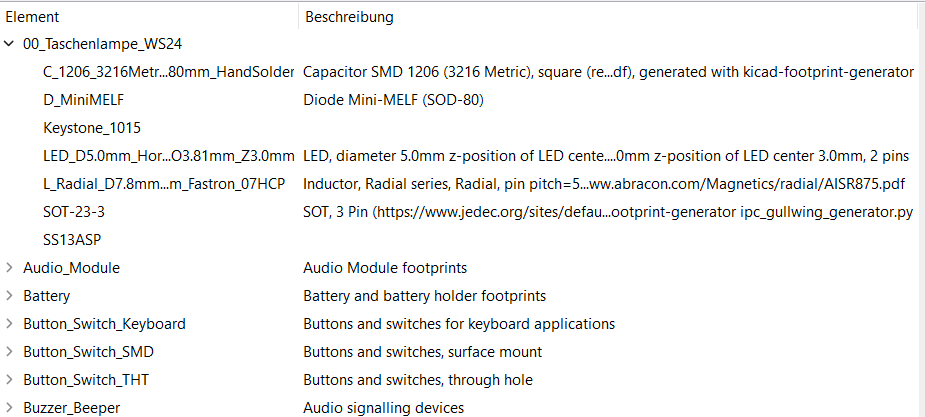
\includegraphics[width=0.8\textwidth]{\figdir/Footprint_Bibliothek mit Bauteilen.png}  
    \caption{Darstellung einer Bibliothek mit Bauteilen.} 
    \label{fig:Abbildung 5} 
\end{figure}  

\subsubsection{Bauteile}  
Ein Schaltplan bildet die Grundlage für jede Leiterplatte.
Die dafür benötigten Bauteile können aus den KiCad-Standardbibliotheken übernommen oder individuell erstellt werden.
Im Workshop wurden alle Bauteile in einer eigenen Bibliothek angelegt, um den Projektanforderungen zu entsprechen.\\
\\
Bauteile werden im Bauteileditor erstellt, wobei Eigenschaften wie Artikelnummern, Datenblätter oder 3D-Modelle hinterlegt werden können.
Um Zeit zu sparen, können bestehende Bauteile kopiert und angepasst werden.  

\begin{figure}[h]  
    \centering  
    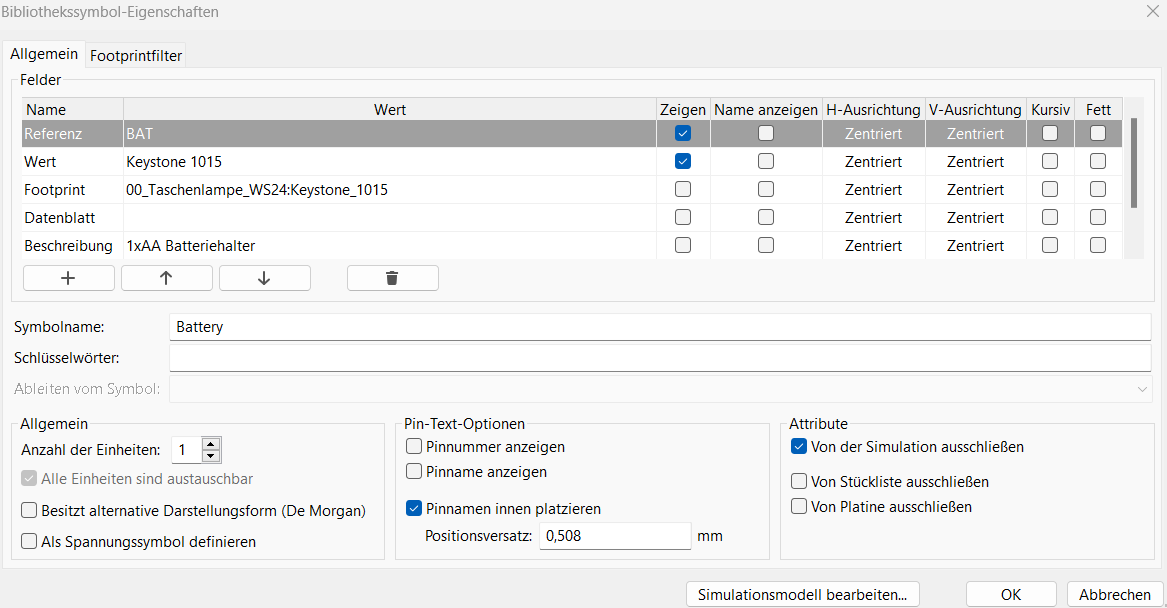
\includegraphics[width=0.8\textwidth, height=5cm]{\figdir/Battery_Symbol Eigenschaften.png}  
    \caption{Eigenschaften eines Bauteils}  
    \label{fig:Abbildung 6}
\end{figure}  

\noindent
Bauteile lassen sich im Bauteileditor entweder komplett neu erstellen oder durch Kopieren bestehender Bauteile zeitsparend anpassen, um sie den individuellen Anforderungen anzupassen.\\
Der folgende Batterie-Halter wurde beispielsweise aus einem Datenblatt übernommen und anschließend entsprechend modifiziert.

\begin{figure}[h]  
    \centering  
    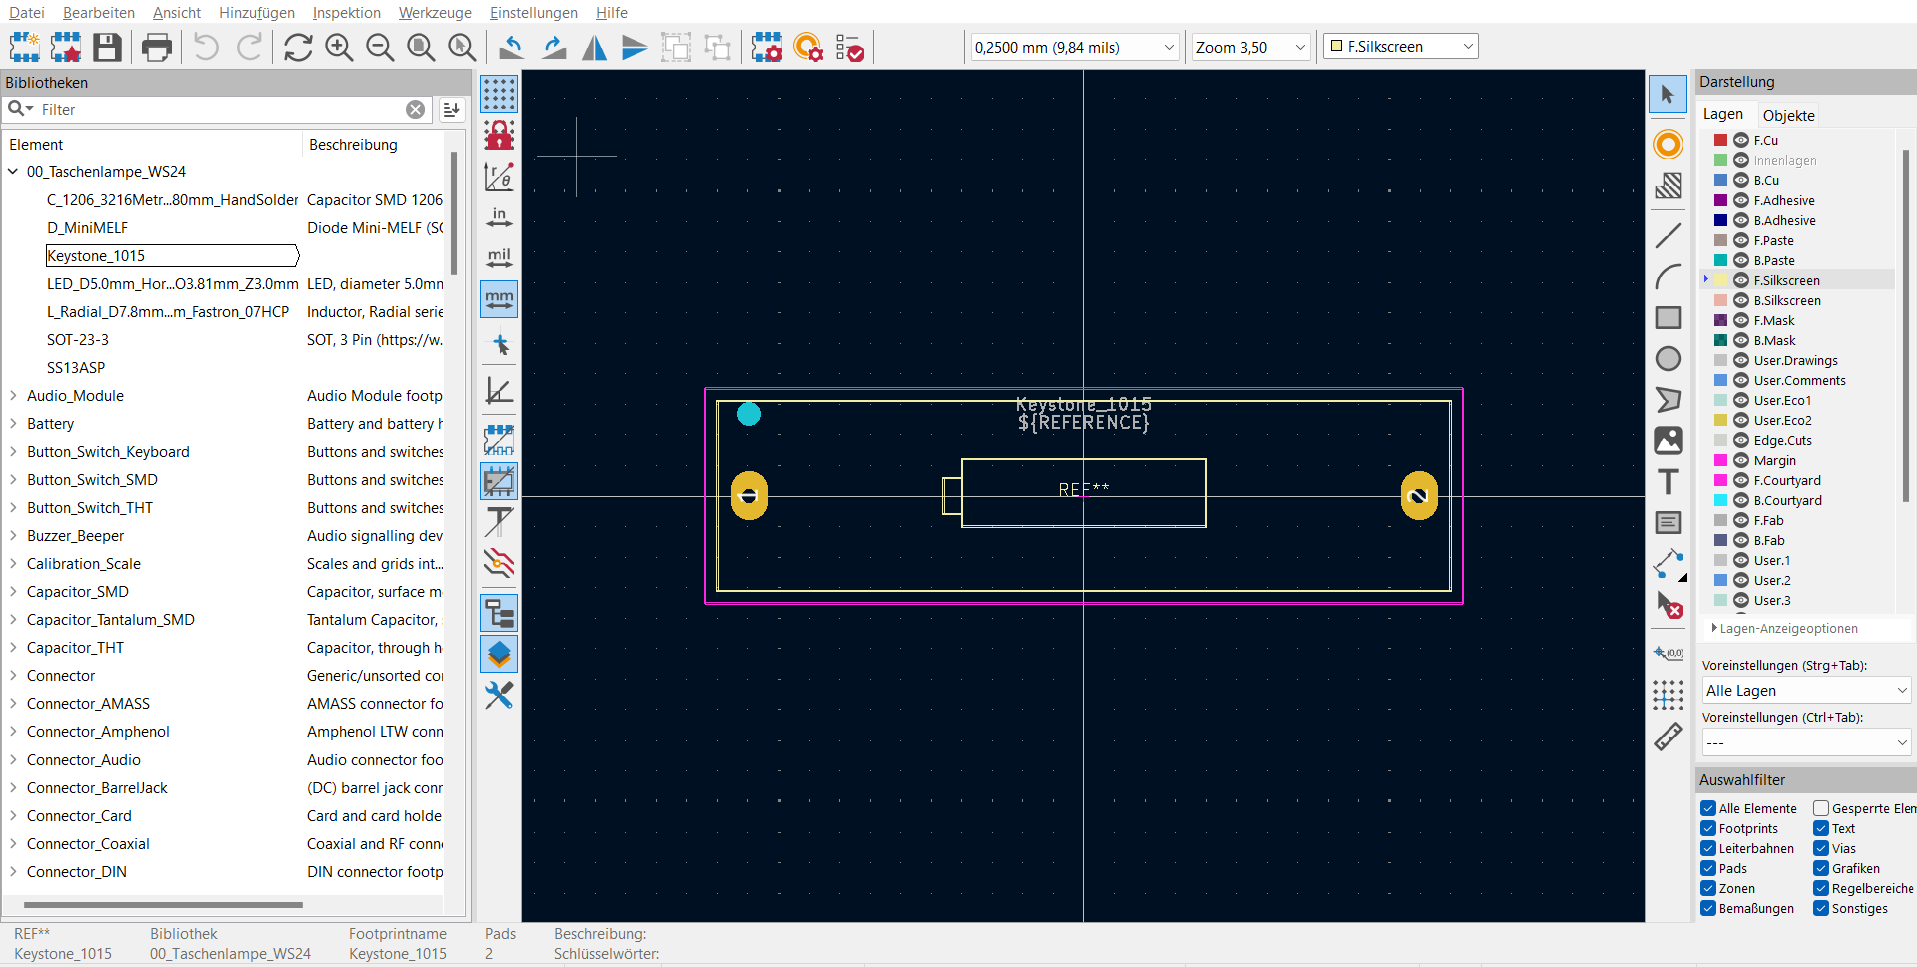
\includegraphics[width=0.8\textwidth, height=5cm]{\figdir/Footprinteditor.png}  
    \caption{Erstellung eines Bauteils im Bauteileditor} 
    \label{fig:Abbildung 7} 
\end{figure}  

\newpage

\subsubsection{Footprints}  
Footprints stellen die Verbindung zwischen den Bauteilen und der Leiterplatte her. Sie werden im Footprinteditor erstellt und repräsentieren den "Fußabdruck" eines Bauteils auf der Platine.\\
\\
Die Verbindung erfolgt über Lötpads, die an die Bauteilkontakte angepasst sind. Für das Handlöten sollten Lötpads größer gestaltet werden, um die Bearbeitung zu erleichtern.
Bei automatischer Bestückung sollten die Pads so klein wie möglich gehalten werden, um Platz zu sparen und den sogenannten Gravestone-Effekt (Aufstellen der Bauteile) zu verhindern.  

\begin{figure}[h]  
    \centering  
    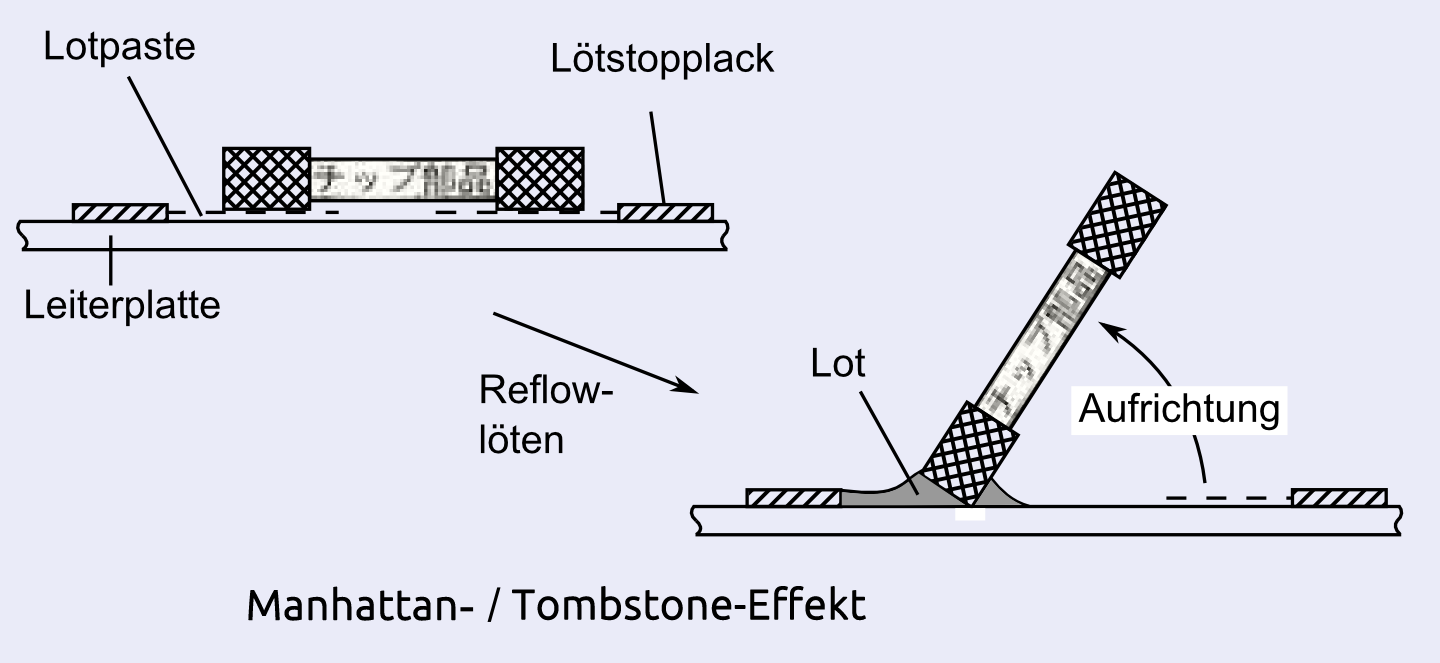
\includegraphics[width=0.6\textwidth, height=4.5cm]{\figdir/Gravestone_Effekt.png}  
    \caption{Gravestone-Effekt: Aufstellen der Bauteile}
    \label{fig:Abbildung 8}  
\end{figure}  
\newpage

\subsection{Erstellen des Schaltplans}  
Nach dem Einpflegen der Bauteile wird der Schaltplan im Schaltplaneditor erstellt. Die Bauteile werden aus der Bibliothek eingefügt, positioniert und miteinander verbunden. Netzklassen können definiert werden, um Abstände zwischen Signalen oder Gruppen (z. B. Last- und Steuerkreis) zu berücksichtigen.\\  
\\
Um die Übersichtlichkeit zu erhöhen, können Textvariablen und Labels genutzt werden. Im Workshop wurden Labels beispielsweise für Ground (GND) eingesetzt.  

\begin{figure}[h]  
    \centering  
    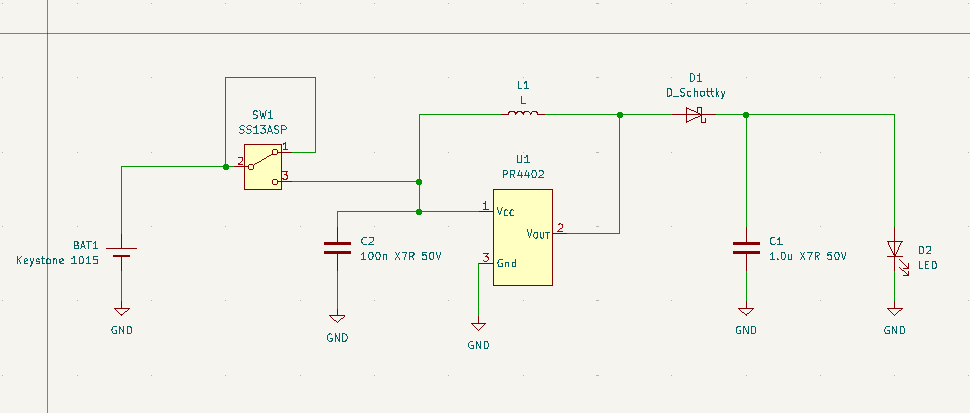
\includegraphics[width=0.8\textwidth]{\figdir/Schaltplan_Taschenlampe.png}  
    \caption{Schaltplan der Taschenlampe mit markierten Labels.}  
    \label{fig:Abbildung 9}
\end{figure}  

\noindent
Wird während der Schaltplanerstellung festgestellt, dass ein Footprint nicht zugewiesen wurde, so kann dies direkt im Schaltplaneditor nachgeholt werden.\\ 
Zur Bearbeitung von Footprints oder Bauteilen kann ebenfalls direkt aus dem Schaltplaneditor in den Footprint- bzw. Bauteileditor gewechselt werden.\\
\\
Während und nach der Schaltplanerstellung sollte ein ERC („Electrical Rule Check“) durchgeführt werden. Dieser Prüfvorgang analysiert den Schaltplan auf Fehler und gibt entsprechende Meldungen aus.
Neben Fehlern können auch Warnungen auftreten, die sich häufig auf Labels oder Netzklassen beziehen. Warnungen sind oft weniger kritisch.
Fehler sollten jedoch nie ohne sorgfältige Prüfung ignoriert werden.
Sollte ein gemeldeter Fehler tatsächlich keinen Einfluss auf die Funktion haben, so kann er im ERC entsprechend markiert und zukünftig ausgeblendet werden.

\newpage

\subsection{Erstellen des Platinenlayouts}  
Das Layout ist die Umwandlung des Schaltplans in eine physische Leiterplattenstruktur. Dabei werden die Footprints der Bauteile auf der Platine positioniert und durch Leiterbahnen verbunden.\\

Der Layoutprozess umfasst die folgenden Schritte:  
\begin{itemize}  
    \item Festlegung der Platinenabmessungen.  
    \item Positionierung der Footprints im Bauraum.  
    \item Manuelles Routen der Leiterbahnen.  
\end{itemize}  

\noindent
Ein durchgehendes GND-Potenzial wird als Kupferschicht ausgeführt. Die restlichen Verbindungen werden manuell erstellt. Dabei ist besonders darauf zu achten, dass die GND-Schicht nicht unterbrochen wird und die Footprints keine Überschneidungen aufweisen.  

\begin{figure}[h]  
    \centering  
    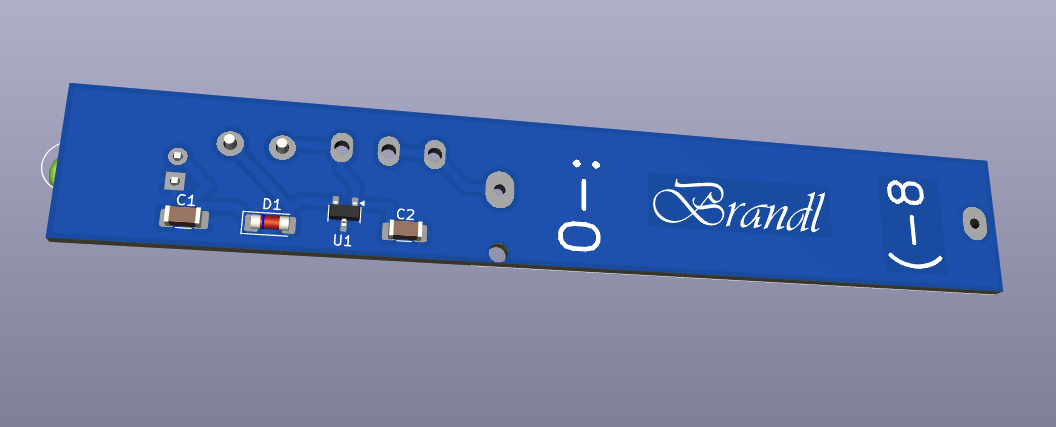
\includegraphics[width=0.8\textwidth]{\figdir/3D_Betrachter_Taschenlampe}  
    \caption{3D Layout Rückseite mit Bauteilen.} 
    \label{fig:Abbildung 10} 
\end{figure}  

\noindent
Die Leiterplatte erhält abschließend einen Bestückungsdruck (Silkscreen), der die Bauteilpositionen markiert.
Dieser kann auch mit optischen Markierungen noch erweitert werden, um das Platinendesign künstlerisch zu gestalten


